	
We define another classification problem that we treat this time with $SVM $.	
In this scenario the parameter to be optimized is C: this parameter can be interpreted as the inverse of $\lambda$, so for small $C$ we will have a smoother solution, while for big $C$ we will only worry about minimizing the mistake.
To do this, as usual, we divide the dataset into two parts: Training Set and Validation Set and execute a cycle on the variable C, memorizing the error defined as the number of wrong classifications. To minimize the variance we repeat the procedure k times.
Once this is done, we look for the error with the lowest number of wrong classifications in the error vector, the corresponding $C$ will be $C_{best}$.	
We repeat, at this point, the calculation performed before using $C_{best}$ instead of $ C $ and plotting the solution.
In the two graphs below we show two cases: in the first, with the same error, we choose the $C_{best}$ lower, so the solution will be smoother, but less precise: there will be many points with $ 0 <\alpha_i<=C$ (we will have a $\underline{w}$ low), while in the second one, with the same error we favor greater $C_{best}$, so the solution will be more complex, but with $\alpha$ vector more sparse.	
\begin{figure}[!ht]
	\centering
	\subfloat[][\emph{Smaller C}.]
	{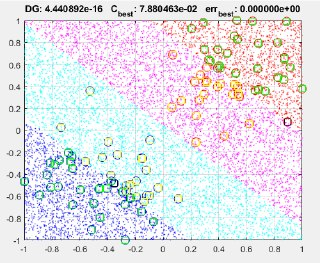
\includegraphics[width=0.4\textwidth]{i6.png}} \quad
	\subfloat[][\emph{Greater C}.]
	{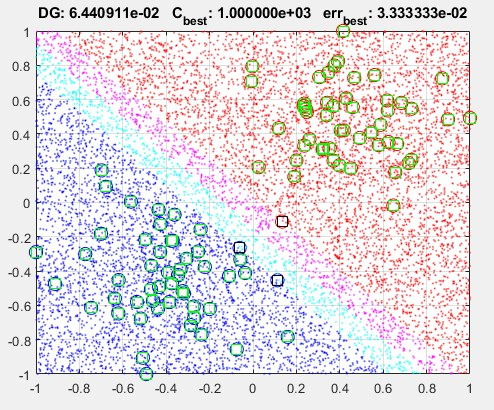
\includegraphics[width=0.4\textwidth]{i7.png}} \\
	
\end{figure}
